\chapter{Практика. Веб-программирование с помощью AllegroServe}
\label{ch:26}

\thispagestyle{empty}

В этой главе вы ознакомитесь с одним из способов разработки веб-приложений на Common Lisp:
используя AllegroServe~-- веб-сервер с открытым исходным кодом. Это не означает, что вы
найдёте здесь исчерпывающее введение в AllegroServe. И я определённо не собираюсь
описывать ничего более, чем небольшую часть огромной темы веб-программирования. Моей целью
является описание достаточного количества базовых вещей по части использования
AllegroServe, которые позволят нам в главе~\ref{ch:29} разработать приложение для
просмотра библиотеки MP3-файлов и проигрывания их на MP3-клиенте. Кроме того, данная глава
может служить кратким введением в веб-программирование для новичков.

\section{30-секундное введение в веб-программирование на стороне сервера}

Хотя в настоящее время веб-программирование обычно означает использование одного из
доступных программных каркасов (frameworks) и различных протоколов, основы
веб-программирования не особо изменились с момента их появления в начале 1990-х. Для
простых приложений, таких как мы напишем в главе~\ref{ch:29}, вам необходимо понять только
несколько основных концепций, так что в этом разделе я сделаю их быстрый обзор. Опытные
веб-программисты могут лишь просмотреть, а то и вовсе пропустить этот
раздел\footnote{Новичкам в веб-программировании, вероятно, понадобится дополнить это
  введение информацией из одного-двух учебников с более глубоким охватом. Вы можете найти
  хорошую подборку доступных online учебников по адресу
  \url{http://www.jmarshall.com/easy/}.}.

Для начала вам необходимо понимание ролей веб-браузера и веб-сервера в
веб-программировании. Хотя современные браузеры поставляются с кучей свистелок и дуделок,
основной функциональностью веб-браузера являются запрос веб-страниц с веб-сервера и их
отображение. Обычно эти страницы пишутся на Hypertext Markup Language (HTML, язык разметки
гипертекста), который указывает браузеру, как отображать страницу, включая информацию о
том, где вставить изображения и ссылки на другие страницы. HTML состоит из текста,
\textit{размеченного} с помощью \textit{тегов}, которые структурируют текст, а эту
структуру браузер использует при отображении страницы. Например, простой HTML-документ
выглядит вот так:

\begin{lstlisting}[language=HTML]
  <html>
    <head>
    <title>Hello</title>
    </head>
    <body>
    <p>Hello, world!</p>
    <p>This is a picture: <img src="some-image.gif"></p>
    <p>This is a <a href="another-page.html">link</a> to another page.</p>
    </body>
  </html>
\end{lstlisting}

Рис.~\ref{fig:26-1}, показывает как браузер отображает эту страницу.

\begin{figure}[htb]
  \centering
  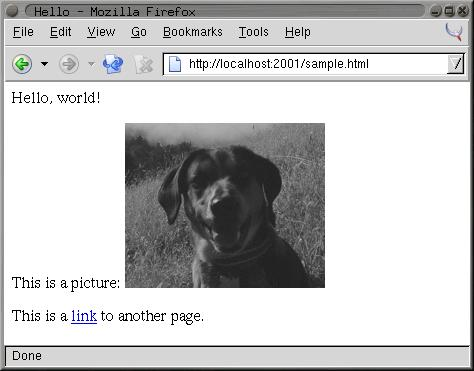
\includegraphics[scale=0.7]{images/new-sample.jpg}
  \label{fig:26-1}
  \caption{Пример веб-страницы}
\end{figure}

Браузер и сервер общаются между собой, используя протокол, называемый Hypertext Transfer
Protocol (HTTP, протокол передачи гипертекста). Хотя вам не нужно беспокоиться
относительно деталей протокола, полезным будет понимание того, что он полностью состоит из
последовательности запросов, инициированных браузером, и ответов, сгенерированных
сервером. Таким образом, браузер подключается к веб-серверу и посылает запрос, который
включает в себя, как минимум, адрес желаемого ресурса (URL) и версию протокола HTTP,
используемую браузером. Браузер также может включать в запрос дополнительные данные; таким
образом браузер отправляет HTML-формы на сервер.

Для ответа на запрос сервер отправляет ответ, состоящий из наборов заголовков и тела
ответа. Заголовки содержат информацию о теле, такую как тип его данных (например, HTML,
обычный текст или изображение), а тело ответа содержит сами данные, которые затем
отображаются браузером. Сервер также может отправлять ответ-ошибку, который сообщит
браузеру о том, что его запрос не может быть обработан по некоторой причине.

И это почти все. После того как браузер получил завершённый ответ от сервера, между
сервером и браузером не происходит никакого общения до тех пор, пока браузер не решит
запросить страницу у сервера в следующий раз\footnote{Загрузка отдельной веб-страницы
  может привести к выполнению множества запросов~-- для отображения HTML-страницы,
  содержащей изображения, браузер должен выполнить отдельный запрос для каждого из них, а
  затем вставить их на соответствующие места страницы.}. Это основное ограничение
веб-программирования~-- для кода, выполняемого на сервере, не существует способа
воздействовать на то, что пользователь увидит в браузере, до тех пор, пока браузер не
сделает новый запрос к серверу\footnote{Большая часть сложности веб-программирования
  заключается в попытках обойти это основное ограничение, чтобы предоставить пользователю
  больше возможностей, таких как интерактивность приложений, выполняющихся на компьютере
  пользователей.}.

Некоторые веб-страницы, называемые \textit{статическими} (\textit{static}) страницами,
являются просто файлами с разметкой на языке HTML, хранимыми на веб-сервере и считываемыми,
когда приходит соответствующий запрос. \textit{Динамические} (\textit{dynamic}) страницы,
с другой стороны, состоят из HTML, генерируемого при каждом запросе страницы
браузером. Например, динамическая страница может быть сгенерирована путём осуществления
запроса к базе данных, а затем конструирования HTML для представления результатов этого
запроса\footnote{К сожалению, слово \textit{динамичный} (\textit{dynamic}) имеет много
  значений в мире веб. Фраза <<динамичный HTML>> (\textit{Dynamic HTML}) относится к HTML,
  который содержит встроенный код, обычно на языке JavaScript, который может выполняться
  браузером без дополнительного общения с сервером. При осторожном использовании
  динамичный HTML может улучшить работу веб-приложения, поскольку даже при использовании
  высокоскоростных соединений выполнение запроса к серверу, получение результата и
  отображение новой страницы может занять заметное количество времени. Что ещё более
  запутывает дело, динамически генерируемые страницы (страницы, генерируемые на сервере)
  могут также содержать динамичный HTML (код для выполнения на клиенте). В этой книге мы
  столкнёмся только с динамически генерируемым обычным, нединамичным HTML.}.

При генерации ответа на запрос код, выполняемый на сервере, получает четыре основные
части информации, на основании которой он работает. Первой является запрошенный адрес
(URL). Но обычно URL используется самим веб-сервером для определения того, какой код
ответствен за генерацию ответа. Затем если URL содержит знак вопроса, то все, что
следует за ним, рассматривается как \textit{строка запроса} (\textit{query string}),
которая обычно игнорируется самим веб-сервером и передаётся им коду, который будет
генерировать ответ. В большинстве случаев строка запроса содержит набор пар
имя/значение. Запрос от браузера может также содержать \textit{POST-данные}, которые также
обычно состоят из пар имя/значение. POST-данные обычно используются для передачи
содержимого форм HTML. Пары имя/значение, переданные либо через строку запроса, либо через
дополнительные данные, обычно называют \textit{параметрами запроса} (\textit{query
  parameters}).

В заключение, для того чтобы связать между собой последовательность отдельных запросов от
одного и того же браузера, код, выполняющийся на сервере, может установить \textit{cookie}
путём отправки специального заголовка в своём ответе браузеру; этот заголовок будет
содержать некий набор данных. После установки cookie браузер будет слать его при каждом
запросе, отправляемом этому серверу. Браузер не заботится о данных, хранимых в cookie,~--
он просто отправляет их обратно на сервер, и код, работающий там, может обрабатывать их
так, как захочет.

Это все базовые элементы, на основании которых основано 99 процентов кода, выполняемого на
веб-сервере. Браузер отправляет запрос, сервер находит код, который будет обрабатывать
запрос, и запускает его, а код использует параметры запроса и cookies для определения
того, что именно нужно сделать.

\section{AllegroServe}

Вы можете отдавать веб-страницы с помощью Common Lisp разными способами; существует, по
крайней мере, три реализации веб-серверов с открытым исходным кодом, написанных на Common
Lisp, а также подключаемые модули, такие как
\pclURL{http://www.fractalconcept.com/asp/html/mod\_lisp.html}{mod\_lisp} и
\pclURL{http://lisplets.sourceforge.net/}{Lisplets}, которые позволяют веб-серверу Apache
или любому контейнеру Java Servlet делигировать обработку запросов серверу Lisp,
работающему в отдельном процессе.

В этой главе мы будем использовать веб-сервер с открытым исходным кодом AllegroServe,
изначально написанный John Foderaro из Franz Inc. AllegroServe включён в версию Allegro,
доступную с сайта Franz для использования с этой книгой. Если вы не используете Allegro,
то вы можете использовать PortableAllegroServe, ответвление (fork) кода AllegroServe,
которое включает в себя уровень (layer) совместимости с Allegro, что позволяет
PortableAllegroServe работать почти на всех реализациях Common Lisp. Код, который мы
напишем в этой главе и в главе~\ref{ch:29}, должен работать как на стандартном
AllegroServe, так и на PortableAllegroServe.

AllegroServe реализует модель программирования, сходную по духу с Java Servlets~-- каждый
раз, когда браузер запрашивает страницу, AllegroServe разбирает запрос и ищет объект,
называемый \textit{сущностью} (\textit{entity}), который будет обрабатывать
запрос. Некоторые классы сущностей, предоставляемые как часть AllegroServe, умеют
обрабатывать статическое содержимое: либо отдельные файлы, либо содержимое
каталога. Другие, которые я буду обсуждать большую часть главы, запускают произвольный код
на Lisp для генерации ответа\footnote{AllegroServe также предоставляет каркас
  (framework), названный \textit{Webactions}, который аналогичен JSP в Java~-- вместо
  написания кода, который генерирует HTML, с помощью Webactions вы можете писать страницы,
  которые являются HTML, но с небольшим количеством специального кода, разворачивающегося
  в настоящий код при обработке страницы. В этой книге я не буду описывать Webactions.}.

Но, перед тем как начать, вам необходимо знать, как запускать AllegroServe и как настроить
его для обработки файлов. Первым шагом является загрузка кода AllegroServe в ваш образ
Lisp. В Allegro вы можете просто набрать \lstinline{(require :aserve)}. В других реализациях
Lisp (а также в Allegro) вы можете загрузить PortableAllegroServe путём загрузки файла
\lstinline{INSTALL.lisp}, находящегося в корне каталога \lstinline{portableaserve}. Загрузка
AllegroServe создаст три новых пакета: \lstinline{NET.ASERVE}, \lstinline{NET.HTML.GENERATOR} и
\lstinline{NET.ASERVE.CLIENT}\footnote{Загрузка PortableAllegroServe также создаст
  дополнительные пакеты для библиотек, обеспечивающих совместимость, но нас в основном
  интересуют три вышеперечисленных пакета.}.

После загрузки сервера вы можете запустить его с помощью функции \lstinline{start} из пакета
\lstinline{NET.ASERVE}. Чтобы иметь простой доступ к символам, экспортированным из пакета
\lstinline{NET.ASERVE}, из пакета \lstinline{COM.GIGAMONKEYS.HTML} (который мы скоро обсудим), а
также остальных частей Common Lisp, нам нужно создать новый пакет:

\begin{myverb}
  CL-USER> (defpackage :com.gigamonkeys.web
              (:use :cl :net.aserve :com.gigamonkeys.html))
  #<The COM.GIGAMONKEYS.WEB package>
\end{myverb}

Теперь переключитесь на этот пакет с помощью следующего выражения \lstinline{IN-PACKAGE}:

\begin{myverb}
  CL-USER> (in-package :com.gigamonkeys.web)
  #<The COM.GIGAMONKEYS.WEB package>
WEB>
\end{myverb} 

Теперь мы можем использовать имена, экспортированные из \lstinline{NET.ASERVE}, без указания
квалификатора. Функция \lstinline{start} запускает сервер. Она принимает множество именованных
параметров, но единственный нужный нам~-- \lstinline{:port}, который указывает номер порта, на
котором сервер будет принимать запросы.  Возможно, вам понадобится использовать большой
номера порта, такой как 2001, вместо порта по умолчанию для HTTP-серверов, 80, поскольку в
Unix-подобных операционных системах только администратор (root) может использовать порты с
номером меньше 1024. Для запуска AllegroServe на порту 80 под Unix вам необходимо
запустить Lisp с правами администратора (root), а затем использовать параметры
\lstinline{:setuid} и \lstinline{:setgid} чтобы заставить \lstinline{start} переключить пользовательский
контекст после открытия этого порта. Вы можете запустить сервер на порту 2001 с помощью
следующей команды:

\begin{myverb}
  WEB> (start :port 2001)
  #<WSERVER port 2001 @ #x72511c72>
\end{myverb}

Теперь сервер выполняется в вашей среде Lisp. Возможно, что при попытке запуска сервера вы
получите ошибку вида <<port already in use>>. Это означает, что данный порт уже
используется каким-то сервером на вашей машине. В таком случае самым простым решением
будет использование другого порта, передав другой аргумент функции \lstinline{start}, а затем
использование нового значения во всех адресах, встречаемых на протяжении данной главы.

Вы можете продолжить взаимодействие с Lisp с помощью REPL, поскольку AllegroServe
запускает отдельные нити для обработки запросов браузеров. Это означает, среди прочего,
что вы можете использовать REPL для того, чтобы заглянуть во <<внутренности>> сервера во
время его работы, что делает тестирование и отладку намного более лёгкой, по сравнению с
тем, когда сервер представляет собой <<чёрный ящик>>.

Предполагая, что вы запустили Lisp на той же машине, где находится и ваш браузер, вы
можете проверить, что сервер запущен, путём перехода в браузере по следующему адресу:
\url{http://localhost:2001/}. В данный момент вы получите в браузере сообщение об ошибке
\lstinline{page-not-found} (страница не найдена), поскольку вы пока ничего не опубликовали. Но
сообщение об ошибке придёт от AllegroServe; это видно по строке внизу страницы. С другой
стороны, если браузер отображает ошибку, сообщающую что-то вроде <<The connection was
refused when attempting to contact localhost:2001>>, то это означает, что сервер не
запущен, или вы запустили его на порту с номером, отличным от 2001.

Теперь мы можем публиковать файлы. Предположим, что у нас есть файл \lstinline{hello.html} в
каталоге \lstinline{/tmp/html} со следующим содержимым:

\begin{lstlisting}[language=HTML]
  <html>
    <head>
    <title>Hello</title>
    </head>
    <body>
    <p>Hello, world!</p>
    </body>
  </html>
\end{lstlisting}

Вы можете опубликовать его с помощью функции \lstinline{publish-file}.

\begin{myverb}
  WEB> (publish-file :path "/hello.html" :file "/tmp/html/hello.html")
  #<NET.ASERVE::FILE-ENTITY @ #x725eddea>
\end{myverb}

Аргумент \lstinline{:path} задаёт путь, который будет использоваться в URL, запрашиваемом
браузером, а аргумент \lstinline{:file} является именем файла на файловой системе. После
вычисления выражения \lstinline{publish-file} вы можете задать в браузере адрес
\url{http://localhost:2001/hello.html}, и он должен отобразить что-то наподобие того, что
изображено на рис.~\ref{fig:26-2}.

\begin{figure}[htb]
  \centering
  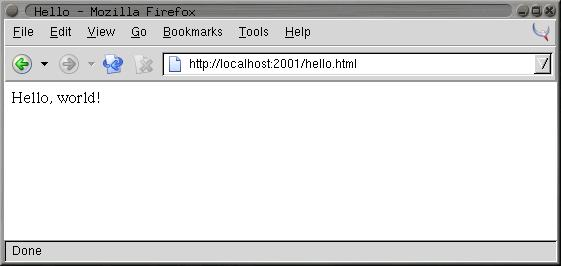
\includegraphics[scale=0.7]{images/hello-world.jpg}
  \label{fig:26-2}
  \caption{\url{http://localhost:2001/hello.html}}
\end{figure}

Вы также можете опубликовать целый каталог с помощью функции \lstinline{publish-directory}. Но
сначала давайте избавимся от уже опубликованной сущности с помощью следующего вызова
\lstinline{publish-file}:

\begin{myverb}
  WEB> (publish-file :path "/hello.html" :remove t)
  NIL
\end{myverb}

Теперь вы можете опубликовать каталог \lstinline{/tmp/html/} целиком (включая его подкаталоги)
с помощью функции \lstinline{publish-directory}.

\begin{myverb}
  WEB> (publish-directory :prefix "/" :destination "/tmp/html/")
  #<NET.ASERVE::DIRECTORY-ENTITY @ #x72625AA2>
\end{myverb}

В данном случае аргумент \lstinline{:prefix} указывает начало пути адресов URL, которые будут
обрабатываться данной сущностью. Так что если сервер получает запрос
\url{http://localhost:2001/foo/bar.html}, то путь будет \lstinline{/foo/bar.html}, который
начинается с \lstinline{/}. Затем этот путь транслируется в имя файла путём замены префикса
(\lstinline{/}) на аргумент \lstinline{:destination} (\lstinline{/tmp/html/}). Так что URL
\url{http://localhost:2001/hello.html} будет преобразован в запрос файла
\lstinline{/tmp/html/hello.html}.

\section{Генерация динамического содержимого с помощью AllegroServe}

Публикация сущностей, генерирующих динамическое содержимое, практически так же проста, как
и публикация статического содержимого. Функции \lstinline{publish} и \lstinline{publish-prefix}
являются <<динамическими>> аналогами \lstinline{publish-file} и
\lstinline{publish-directory}. Основная их идея заключается в том, что вы публикуете функцию,
которая будет вызываться для генерации ответа на запрос либо к определённому адресу
(URL), либо к любому адресу с заданным префиксом. Эта функция будет вызвана с двумя
аргументами: объектом, представляющим запрос, и опубликованной сущностью. Большую часть
времени нам не нужно будет ничего делать с опубликованной сущностью, за исключением её
передачи набору макросов, которые вскоре будут описаны. С другой стороны, мы будем
использовать объект запроса для получения информации, переданной браузером: параметров
запроса, переданных в строке URL, или данных, посланных формами HTML.

В качестве простого примера использования функции для генерации динамического
содержимого давайте напишем функцию, которая будет генерировать страницу с различными
случайными числами при каждом обращении к ней.

\begin{myverb}
  (defun random-number (request entity)
    (with-http-response (request entity :content-type "text/html")
      (with-http-body (request entity)
        (format 
         (request-reply-stream request)
         "<html>~@
          <head><title>Random</title></head>~@
          <body>~@
          <p>Random number: ~d</p>~@
          </body>~@
          </html>~@
         "
         (random 1000)))))
\end{myverb}

Макросы \lstinline{with-http-response} и \lstinline{with-http-body} являются частью
AllegroServe. Первый из макросов начинает процесс генерации ответа HTTP и может быть
использован, так же как в нашем примере, для указания таких вещей, как тип возвращаемых
данных. Он также обрабатывает различные требования, указанные в стандарте HTTP, такие как
обработка запросов \lstinline{If-Modified-Since}. Макрос же \lstinline{with-http-body} фактически
отправляет заголовки HTTP-ответа, а затем вычисляет своё тело, которое должно содержать
код, генерирующий содержимое ответа. Внутри \lstinline{with-http-response}, но перед
\lstinline{with-http-body} вы можете добавить или изменить значение заголовков HTTP, которые
будут отправлены в ответе. Функция \lstinline{request-reply-stream} также является частью
AllegroServe и возвращает поток, в который вы должны записывать данные, предназначенные для
отправления браузеру.

Как видно из этой функции, вы можете просто использовать \lstinline{FORMAT} для вывода HTML в
поток, возвращённый вызовом \lstinline{request-reply-stream}. В следующем разделе я покажу вам
более удобные способы программной генерации HTML\footnote{Спецификатор \lstinline{~@}, за
  которым следует знак новой строки, заставляет \lstinline{FORMAT} игнорировать пробельные
  знаки после этого знака новой строки, что позволяет вам красиво отформатировать код без
  фактического добавления пробельных знаков в HTML. Поскольку пробельные знаки обычно не
  являются значимыми в HTML, это никак не влияет не работу браузера, но делает
  сгенерированный код HTML более удобным для чтения людьми.}.

Теперь мы готовы к публикации данной функции.

\begin{myverb}
  WEB> (publish :path "/random-number" :function 'random-number)
  #<COMPUTED-ENTITY @ #x7262bab2>
\end{myverb}

Так же как и в функции \lstinline{publish-file}, аргумент \lstinline{:path} указывает <<путевую
часть>> (path part) адреса, указание которой будет приводить к вызову данной функции.
Аргумент \lstinline{:function} указывает либо имя функции, либо сам функциональный объект.
Использование имени функции, как показано в этом примере, позволяет вам в дальнейшем
переопределить функцию, не выполняя заново процесса публикации, для того чтобы AllegroServe
стал использовать новое определение. После вычисления данного вызова вы можете указать в
браузере адрес http://localhost:2001/random-number для получения страницы со случайным
числом, как это показано на рис.~\ref{fig:26-3}.

\begin{figure}[htb]
  \centering
  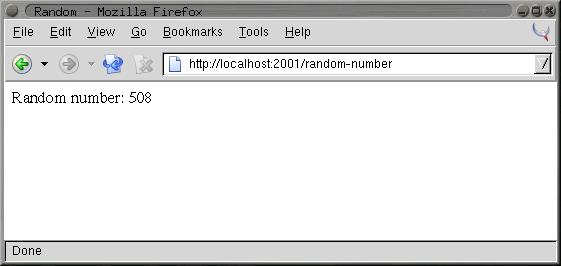
\includegraphics[scale=0.7]{images/random-number.jpg}
  \label{fig:26-3}
  \caption{\url{http://localhost:2001/random-number}}
\end{figure}

\section{Генерация HTML}

Хотя использование \lstinline{FORMAT} для генерации HTML вполне приемлемо для
генерации простых страниц наподобие приведённой выше, по мере того как вы начнёте
создавать более сложные, было бы лучше иметь более краткий способ генерации HTML. Для
генерации HTML из представления в виде s-выражений существует несколько библиотек,
включая \lstinline{htmlgen}, которая поставляется вместе с AllegroServe. В~этой главе мы будем
применять библиотеку FOO\footnote{FOO~-- это рекурсивный тавтологический
  акроним для <<FOO Outputs Output>>.}, которая использует примерно ту же модель, что и
\texttt{htmlgen}, и чью реализацию мы рассмотрим более подробно в главах~\ref{ch:30}
и~\ref{ch:31}. Сейчас, однако, нам нужно лишь знать, как использовать FOO.

Генерирование HTML из Lisp вполне естественно, так как s-выражения и HTML по своему
существу изоморфны. Мы можем представить HTML-элементы с помощью s-выражений, рассматривая
каждый элемент HTML как список, <<помеченный>> соответствующим первым элементом, таким как
ключевым символом с таким же именем, что имеет тег HTML. Таким образом, HTML
\lstinline!<p>foo</p>! представляется s-выражением \lstinline{(:p "foo")}. Так как элементы
HTML, так же как и списки в s-выражениях, могут быть вложенными, эта схема распространяется
и на более сложный HTML. Для примера вот такой HTML:

\begin{lstlisting}[language=HTML]
  <html>
    <head>
    <title>Hello</title>
    </head>
    <body>
    <p>Hello, world!</p>
    </body>
  </html>
\end{lstlisting}

\noindent{}может быть представлен в виде следующего s-выражения:

\begin{myverb}
  (:html
    (:head (:title "Hello"))
    (:body (:p "Hello, world!")))
\end{myverb}

Элементы HTML с атрибутами несколько усложняют дело, но не создают непреодолимых
проблем. FOO предоставляет два способа включения атрибут в тег. Одним из них
является добавление после первого элемента списка пар ключ/значение. Первый же элемент,
который следует за парами ключ/значение и который сам не является ключевым символом,
обозначает начало содержимого элемента. Таким образом, такой HTML:

\begin{lstlisting}[language=HTML]
  <a href="foo.html">This is a link</a>
\end{lstlisting}

\noindent{}будет представляться следующим s-выражением:

\begin{myverb}
  (:a :href "foo.html" "This is a link")
\end{myverb}

Другой предоставляемый FOO синтаксис заключается в группировке имени тега и его
атрибутов в отдельный список следующим образом:

\begin{myverb}
  ((:a :href "foo.html") "This is link.")
\end{myverb}

FOO может использовать представление HTML в виде s-выражений двумя
способами. Функция \lstinline{emit-html} получает представляющее HTML s-выражение и выводит
соответствующий HTML.

\begin{myverb}
  WEB> (emit-html '(:html (:head (:title "Hello")) (:body (:p "Hello, world!"))))
  <html>
    <head>
      <title>Hello</title>
    </head>
    <body>
      <p>Hello, world!</p>
    </body>
  </html>
  T
\end{myverb}

Однако \lstinline{emit-html} не всегда является наиболее эффективным способом генерации
HTML, так как её аргументом должно быть законченное s-выражение, предоставляющее HTML,
который нужно сгенерировать. Хотя генерировать такое представление легко, действовать так
не всегда эффективно. Например, представим, что нам нужно сгенерировать страницу HTML,
содержащую список из 10~000 случайных чисел. Мы можем построить соответствующее
s-выражение, используя шаблон квазицитирования, а затем передать его в функцию
\lstinline{emit-html}:

\begin{myverb}
  (emit-html
    `(:html
       (:head
         (:title "Random numbers"))
       (:body 
         (:h1 "Random numbers")
         (:p ,@(loop repeat 10000 collect (random 1000) collect " ")))))
\end{myverb}

Однако этот код должен построить дерево, содержащее 10000-элементный список, перед тем как
он сможет даже начать генерировать HTML, и все это s-выражение станет мусором, как только
HTML будет сгенерирован. Для избежания такой неэффективности FOO также
предоставляет макрос \lstinline{html}, позволяющий вам встраивать произвольный код Lisp в
середину s-выражения, по которому будет генерироваться HTML.

Литеральные значения, такие как строки и числа, входа \lstinline{html} будут подставлены в
генерируемый HTML. Также символы интерпретируются как ссылки на переменные, которые они
именуют, и сгенерированный код будет брать их значения во время выполнения. Таким образом,
оба следующих выражения:

\begin{myverb}
  (html (:p "foo"))

  (let ((x "foo")) (html (:p x)))
\end{myverb}

\noindent{}сгенерируют следующее:

\begin{lstlisting}[language=HTML]
  <p>foo</p>
\end{lstlisting}

Формы списков, которые не начинаются с ключевых символов, рассматриваются как код и
встраиваются в генерируемый код. Любые значения, возращаемые встроенным кодом, будут
проигнорированы, но такой код сам может генерировать HTML путём вызова
\lstinline{html}. Например, для генерации содержимого списка в виде HTML мы можем написать
следующее:

\begin{myverb}
  (html (:ul (dolist (item (list 1 2 3)) (html (:li item)))))
\end{myverb}

\noindent{}что сгенерирует следующий HTML:

\begin{lstlisting}[language=HTML]
  <ul>
    <li>1</li>
    <li>2</li>
    <li>3</li>
  </ul>
\end{lstlisting}

Если вы захотите выдать значение формы, вы должны обернуть его в псевдотег
\lstinline{:print}. Таким образом, выражение

\begin{myverb}
  (html (:p (+ 1 2)))
\end{myverb}

\noindent{}сгенерирует такой HTML после вычисления и отбрасывания значения \lstinline{3}:

\begin{lstlisting}[language=HTML]
  <p></p>
\end{lstlisting}

Для выдачи \lstinline{3} вы должны написать такой код:

\begin{myverb}
  (html (:p (:print (+ 1 2))))
\end{myverb}

Или же вы можете вычислить значение и сохранить его в переменной вне вызова \lstinline{html}
следующим образом:

\begin{myverb}
(let ((x (+ 1 2))) (html (:p x)))
\end{myverb}

Таким образом вы можете использовать макрос \lstinline{html} для генерации списка случайных
чисел следующим образом:

\begin{myverb}
  (html
    (:html
      (:head
        (:title "Random numbers"))
      (:body 
        (:h1 "Random numbers")
        (:p (loop repeat 10 do (html (:print (random 1000)) " "))))))
\end{myverb}

Версия, использующая макрос \lstinline{html}, будет эффективнее, чем использующая
\lstinline{emit-html}. И не только из-за того, что теперь не нужно генерировать s-выражение,
представляющее страницу целиком, но и из-за того, что большая часть работы по
интерпретации s-выражения, которую \lstinline{emit-html} осуществляет во время выполнения,
будет сделана однократно, во время раскрытия макроса, а не каждый раз при выполнении кода.

Вы можете управлять тем, куда будет отправлен вывод \lstinline{html} и \lstinline{emit-html}, с
помощью макроса \lstinline{with-html-output}, который также является частью библиотеки
FOO. Вы можете использовать макросы \lstinline{with-html-output} и \lstinline{html} для
переписывания \lstinline{random-number} следущим образом:

\begin{myverb}
  (defun random-number (request entity)
    (with-http-response (request entity :content-type "text/html")
      (with-http-body (request entity)
        (with-html-output ((request-reply-stream request))
          (html
            (:html
              (:head (:title "Random"))
              (:body
                (:p "Random number: " (:print (random 1000))))))))))
\end{myverb}

\section{Макросы HTML}

Другой возможностью FOO является то, что он позволяет вам определять <<макросы>>
HTML, которые могут преобразовывать произвольные формы в представляющие HTML s-выражения,
которые понимает макрос \lstinline{html}. Например, предположим, что вы заметили, что часто
создаёте страницы следующего вида:

\begin{myverb}
  (:html
    (:head (:title "Some title"))
    (:body
      (:h1 "Some title")
      ... stuff ...))
\end{myverb}

Вы можете определить макрос HTML, представляющий этот образец, следующим образом:

\begin{myverb}
  (define-html-macro :standard-page ((&key title) &body body)
    `(:html
       (:head (:title ,title))
       (:body
        (:h1 ,title)
        ,@body)))
\end{myverb}

Теперь вы можете использовать <<тег>> \lstinline{:standard-page} в ваших представляющих HTML
s-выражениях, и он будет раскрыт перед интерпретацией или компиляцией этих выражений.
Например, следующий код:

\begin{myverb}
  (html (:standard-page (:title "Hello") (:p "Hello, world.")))
\end{myverb}

\noindent{}сгенерирует такой HTML:

\begin{lstlisting}[language=HTML]
  <html>
    <head>
      <title>Hello</title>
    </head>
    <body>
      <h1>Hello</h1>
      <p>Hello, world.</p>
    </body>
  </html>
\end{lstlisting}

\section{Параметры запроса}

Конечно, генерация HTML является только половиной темы web-программирования. Ещё одной
вещью, которую вы должны уметь делать, является получение ввода от пользователя. Как я
рассказывал в разделе <<30-секундное введение в web-программирование на стороне сервера>>,
когда браузер запрашивает страницу у web-сервера, он может послать параметры запроса в
адресе URL или POST-данные, и оба этих источника рассматриваются как ввод для кода на
стороне сервера.

AllegroServe, как и большинство других каркасов web-программирования, берёт на себя заботу
о разборе обоих этих источников ввода для вас. В то время когда ваша опубликованная
функция вызывается, все пары ключ/значение из строки запроса и/или POST-данных уже
декодированы и помещены в ассоциативный список (alist), который вы можете получить из
объекта запроса с помощью функции \lstinline{request-query}. Следующая функция возвращает
страницу, отображающую все полученные ею параметры запроса:

\begin{myverb}
  (defun show-query-params (request entity)
    (with-http-response (request entity :content-type "text/html")
      (with-http-body (request entity)
        (with-html-output ((request-reply-stream request))
          (html
            (:standard-page
             (:title "Query Parameters")
             (if (request-query request)
               (html 
                 (:table :border 1
                         (loop for (k . v) in (request-query request)
                            do (html (:tr (:td k) (:td v))))))
               (html (:p "No query parameters.")))))))))

  (publish :path "/show-query-params" :function 'show-query-params)
\end{myverb}

Если вы укажете своему браузеру URL со строкой запроса, подобной такой:

\begin{myverb}
  http://localhost:2001/show-query-params?foo=bar&baz=10
\end{myverb}

\noindent{}вы получите страницу, подобную показанной на рис.~\ref{fig:26-4}.

\begin{figure}[htb]
  \centering
  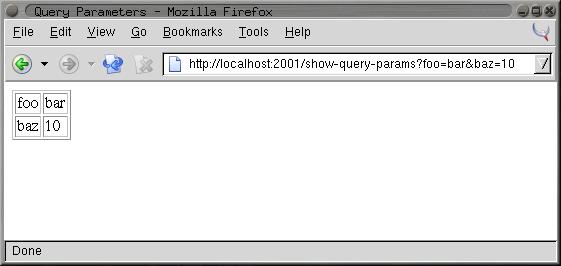
\includegraphics[scale=0.7]{images/show-query-params-1a.jpg}
  \label{fig:26-4}
  \caption{\url{http://localhost:2001/show-query-params?foo=bar&baz=10}}
\end{figure}

Для генерации POST-данных нам нужна форма HTML. Следующая функция генерирует простую
форму, которая посылает свои данные show-query-params:

\begin{myverb}
  (defun simple-form (request entity)
    (with-http-response (request entity :content-type "text/html")
      (with-http-body (request entity)
        (let ((*html-output* (request-reply-stream request)))
          (html
            (:html
              (:head (:title "Simple Form"))
              (:body
               (:form :method "POST" :action "/show-query-params"
                 (:table
                  (:tr (:td "Foo")
                       (:td (:input :name "foo" :size 20)))
                  (:tr (:td "Password")
                       (:td (:input :name "password" :type "password" :size 20))))
                 (:p (:input :name "submit" :type "submit" :value "Okay")
                     (:input ::type "reset" :value "Reset"))))))))))

  (publish :path "/simple-form" :function 'simple-form)
\end{myverb}

Перейдите в вашем браузере по адресу \url{http://localhost:2001/simple-form}~-- вы должны
увидеть страницу, подобную изображённой на рис.~\ref{fig:26-5}.

\begin{figure}[htb]
  \centering
  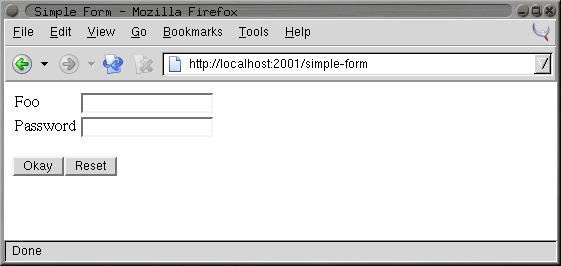
\includegraphics[scale=0.7]{images/simple-form.jpg}
  \label{fig:26-5}
  \caption{\url{http://localhost:2001/simple-form}}
\end{figure}

Если вы заполните форму значениями <<abc>> и <<def>>, щёлкните на кнопку \texttt{Okay}, то
получите страницу, сходную с изображённой на рис.~\ref{fig:26-6}.

\begin{figure}[htb]
  \centering
  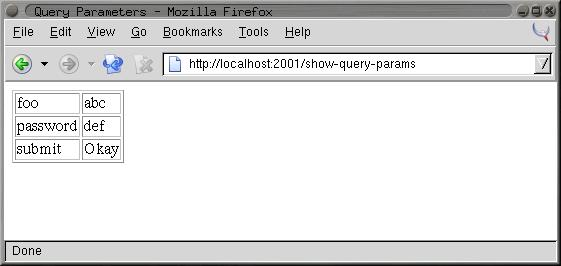
\includegraphics[scale=0.7]{images/show-query-params-2.jpg}
  \label{fig:26-6}
  \caption{Результат посылки простой формы}
\end{figure}

Однако чаще всего вам не нужно проходить по всем параметрам запроса: обычно вам нужно
просто получить определённый параметр. Например, вы можете захотеть модифицировать
\lstinline{random-number} так, чтобы предельное значение, передаваемое в функцию
\lstinline{RANDOM}, предоставлялось как параметр запроса. В таком случае используется функция
\lstinline{request-query-value}, получающая объект запроса и имя параметра, значение которого
вы хотите получить. Она возвращает либо значение параметра в виде строки, либо
\lstinline{NIL}, если такой параметр не предоставлен. <<Параметризованная>> версия
\lstinline{random-number} может выглядеть следующим образом:

\begin{myverb}
  (defun random-number (request entity)
    (with-http-response (request entity :content-type "text/html")
      (with-http-body (request entity)
        (let* ((*html-output* (request-reply-stream request))
               (limit-string (or (request-query-value "limit" request) ""))
               (limit (or (parse-integer limit-string :junk-allowed t) 1000)))
          (html
            (:html
              (:head (:title "Random"))
              (:body
                (:p "Random number: " (:print (random limit))))))))))
\end{myverb}

Так как \lstinline{request-query-value} может возвращать как \lstinline{NIL}, так и пустую
строку, мы должны обрабатывать оба этих случая при разборе параметра и его преобразования
в число, которое будет передано \lstinline{RANDOM}. Мы можем обработать значение
\lstinline{NIL} при связывании переменной \lstinline{limit-string}, связывая её с
пустой строкой (\lstinline{""}), если параметра \lstinline{"limit"} нет. Затем мы можем использовать
аргумент функции \lstinline{PARSE-INTEGER} \lstinline{:junk-allowed} для гарантии того,
что она вернёт либо \lstinline{NIL} (если не сможет разобрать целое число из переданной
строки), либо целое число. В разделе <<Небольшой каркас приложений>> мы разработаем
несколько макросов для облегчения работы по получению параметров запроса и преобразованию
их в различные типы.

\section{Cookies}

В AllegroServe вы можете послать заголовок \lstinline{Set-Cookie}, который укажет браузеру
сохранить cookie и посылать его со всеми последующими запросами, путём вызова функции
\lstinline{set-cookie-header} внутри тела \lstinline{with-http-response}, но перед вызовом
\lstinline{with-http-body}. Первый аргумент этой функции должен быть объектом запроса, а
остальные аргументы~-- ключевые аргументы, используемые для установки различных свойств
cookie. Обязательными являются лишь два аргумента: \lstinline{:name} и \lstinline{:value}, оба из
которых являются строками. Остальные возможные аргументы, влияющие на посылаемый браузеру
cookie: \lstinline{:expires}, \lstinline{:path}, \lstinline{:domain} и \lstinline{:secure}.

Из этих аргументов нам следует обратить внимание лишь на \lstinline{:expires}. Он управляет
тем, как долго браузер должен сохранять cookie. Если \lstinline{:expires} равен \lstinline{NIL}
(по умолчанию), браузер сохранит cookie только до завершения своей работы. Другие
возможные значения: \lstinline{:never}, что означает, что cookie должен сохраняться навсегда,
или всемирное (universal) время, как возвращается \lstinline{GET-UNIVERSAL-TIME} или
\lstinline{ENCODE-UNIVERSAL-TIME}. Значение \lstinline{:expires}, равное нулю, указывает клиенту
немедленно удалить существующие cookie\footnote{За информацией о смысле остальных
  параметров обращайтесь к документации AllegroServe и RFC 2109, разъясняющей механизм
  cookie.}.

После того как вы установили cookie, вы можете использовать функцию
\lstinline{get-cookie-values} для получения ассоциативного списка (alist), содержащего по паре
имя/значение на каждый cookie, посланный браузером. Из этого списка вы можете получить
значения отдельных cookie с помощью \lstinline{ASSOC} и \lstinline{CDR}.

Следующая функция отображает имена и значения всех cookie, посланных браузером:

\begin{myverb}
  (defun show-cookies (request entity)
    (with-http-response (request entity :content-type "text/html")
      (with-http-body (request entity)
        (with-html-output ((request-reply-stream request))
          (html
            (:standard-page
             (:title "Cookies")
             (if (null (get-cookie-values request))
               (html (:p "No cookies."))
               (html 
                 (:table
                   (loop for (key . value) in (get-cookie-values request)
                      do (html (:tr (:td key) (:td value)))))))))))))

  (publish :path "/show-cookies" :function 'show-cookies)
\end{myverb}

При первой загрузке страницы \lstinline{http://localhost:2001/show-cookies} она должна
отобразить сообщение \lstinline{"No cookies"}, как показано на рис.~\ref{fig:26-7}, так как
вы ещё ничего не установили.

\begin{figure}[htb]
  \centering
  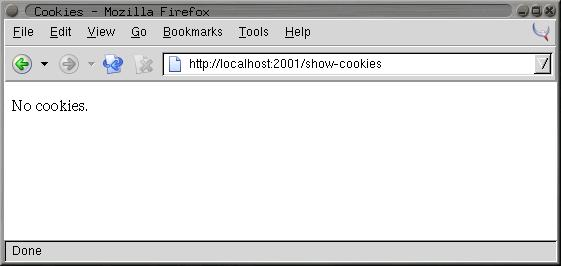
\includegraphics[scale=0.7]{images/show-cookies-no-cookies.jpg}
  \label{fig:26-7}
  \caption{\url{http://localhost:2001/show-cookies} без установленных cookie}
\end{figure}

Для установки cookie нам понадобится другая функция, такая как эта:

\begin{myverb}
  (defun set-cookie (request entity)
    (with-http-response (request entity :content-type "text/html")
      (set-cookie-header request :name "MyCookie" :value "A cookie value")
      (with-http-body (request entity)
        (with-html-output ((request-reply-stream request))
          (html 
            (:standard-page
             (:title "Set Cookie")
             (:p "Cookie set.")
             (:p (:a :href "/show-cookies" "Look at cookie jar."))))))))

  (publish :path "/set-cookie" :function 'set-cookie)
\end{myverb}

Если вы откроете в браузере \url{http://localhost:2001/set-cookie}, он должен отобразить
страницу, показанную на рис.~\ref{fig:26-8}. Вдобавок сервер пошлёт заголовок
\lstinline{Set-Cookie} с cookie по имени <<MyCookie>> со значением <<A cookie value>>. Если вы
нажмёте на ссылку //Look at cookie jar//, то попадёте на страницу \lstinline{/show-cookies},
где увидите новый cookie, как показано на рис.~\ref{fig:26-9}. Так как вы не задали
аргумент \lstinline{:expires}, браузер продолжит посылать cookie при каждом запросе, пока вы не
выйдете из него.

\begin{figure}[htb]
  \centering
  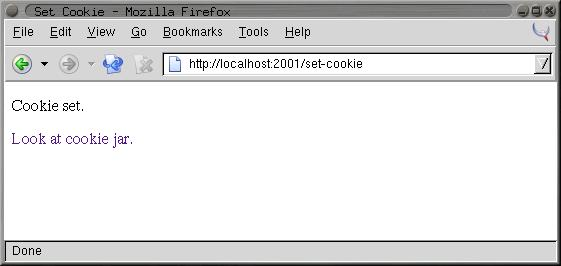
\includegraphics[scale=0.7]{images/set-cookie.jpg}
  \label{fig:26-8}
  \caption{\url{http://localhost:2001/set-cookie}}
\end{figure}

\begin{figure}[htb]
  \centering
  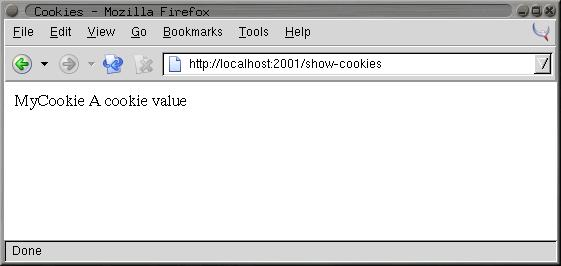
\includegraphics[scale=0.7]{images/show-cookies-one-cookie.jpg}
  \label{fig:26-9}
  \caption{\url{http://localhost:2001/show-cookies} после установки cookie}
\end{figure}

\section{Небольшой каркас приложений}

Хотя AllegroServe предоставляет достаточно прямой доступ ко всем базовым возможностям,
необходимым для написания кода, выполняющегося на стороне сервера (доступ к параметрам
запроса как из строки запроса, так и из POST-данных; возможность установки cookie и
получения их значений; и, конечно же, возможность генерации ответа для посылки
браузеру), приходится писать некоторое количество раздражающе повторяющегося кода.

Например, каждая генерирующая HTML-функция, которую вы будете писать, будет получать в
качестве аргументов запрос и сущность, а затем будет содержать вызовы
\lstinline{with-http-response}, \lstinline{with-http-body} и, если вы будете использовать FOO
для генерирации HTML, \lstinline{with-html-output}. Далее функции, которым нужно получать
параметры запроса, будут содержать множество вызовов \lstinline{request-query-value} и ещё
больше кода для преобразования получаемых строк к нужным типам. И наконец, вам нужно не
забыть опубликовать функции.

Для уменьшения повторяющегося кода, который вам нужно писать, мы можем реализовать
небольшой каркас поверх AllegroServe в целях облегчения определения функций,
обрабатывающих запросы по определённым URL.

Базовым приближением будет определение макроса \lstinline{define-url-function}, который мы будем
использовать для определения функций, которые будут автоматически публиковаться с помощью
\lstinline{publish}. Этот макрос будет раскрываться в \lstinline{DEFUN}, содержащий
соответствующий шаблонный код, а также в код публикации функции под URL с таким же, как у
функции, именем. Он также возьмёт на себя заботу по генерации кода извлечения значений
параметров запроса и cookies и связывания их с переменными, объявленными в списке
параметров функции. Таким образом, базовой формой определения \lstinline{define-url-function}
будет такая:

\begin{myverb}
  (define-url-function name (request query-parameter*)
    body)
\end{myverb}

\noindent{}где \lstinline{body} будет кодом, выдающим код HTML-страницы. Он будет обернут в вызов макроса
\lstinline{html} из FOO и поэтому для простых страниц может не содержать ничего, кроме
представляющего HTML s-выражения.

Внутри тела переменные параметров запроса будут связаны со значениями параметров запроса с
такими же именами или значениями cookie. В простейшем случае значением параметра запроса
будет строка, полученная из параметра запроса или поля POST-данных с таким же именем. Если
же параметр запроса задаётся списком, вы также можете задать автоматическое преобразование
типа, значение по умолчанию и то, нужно ли получать значение параметра из cookie и сохранять его
в cookie. Полный синтаксис для параметра запроса выглядит так:

\begin{myverb}
  name | (name type [default-value] [stickiness])
\end{myverb}

\lstinline{type} должен быть именем, распознаваемым \lstinline{define-url-function}. Мы скоро
обсудим, как определять новые типы. \lstinline{default-value} должно быть значением данного
типа. И наконец, \lstinline{stickness}, если предоставлен, указывает, что значение параметра
должно быть взято из cookie с соответствующим именем в случае, если параметр запроса не
предоставлен, а также что в ответе должен быть послан заголовок \lstinline{Set-Cookie}, который
сохранит значение cookie с этим именем. Таким образом, сохраняемый параметр (sticky
parameter), после явного предоставления значения в параметре запроса, сохранит это
значение при последующих запросах страницы, даже если параметр запроса не предоставляется.

Имя используемого cookie зависит от значения \lstinline{stickness}: при значении \lstinline{:global}
cookie будет иметь то же имя, что и параметр. Таким образом, различные функции,
использующие глобальные сохраняемые параметры с одинаковым именем, будут разделять
значение. Если \lstinline{stickness} равно \lstinline{:package}, то имя cookie будет сконструировано
из имён параметра и пакета, в котором находится имя функции; это позволит функциям одного
пакета разделять значения, не заботясь о возможных конфликтах с параметрами функций других
пакетов. И наконец, параметр со значением \lstinline{stickness}, равным \lstinline{:local}, будет
использовать имя cookie, составленное из имён параметра, пакета, в котором находится имя
функции, и самого имени функции, что делает его уникальным для этой функции.

Например, вы можете использовать \lstinline{define-url-function} для замены предыдущего
11-строчного определения \lstinline{random-page} 5-строчной версией:

\begin{myverb}
  (define-url-function random-number (request (limit integer 1000))
    (:html
      (:head (:title "Random"))
      (:body
        (:p "Random number: " (:print (random limit))))))
\end{myverb}

Если вы хотите, чтобы аргумент \lstinline{limit} сохранялся, то должны изменить объявление
\lstinline{limit} следующим образом: \lstinline{(limit integer 1000 :local)}.

\section{Реализация}

Я разъясню реализацию \lstinline{define-url-function} <<сверху вниз>>. Сам макрос выглядит
следующим образом:

\begin{myverb}
  (defmacro define-url-function (name (request &rest params) &body body)
    (with-gensyms (entity)
      (let ((params (mapcar #'normalize-param params)))
        `(progn
           (defun ,name (,request ,entity)
             (with-http-response (,request ,entity :content-type "text/html")
               (let* (,@(param-bindings name request params))
                 ,@(set-cookies-code name request params)
                 (with-http-body (,request ,entity)
                   (with-html-output ((request-reply-stream ,request))
                     (html ,@body))))))
           (publish :path ,(format nil "/~(~a~)" name) :function ',name)))))
\end{myverb}

Давайте рассмотрим её по шагам, начиная с первых строк.

\begin{myverb}
  (defmacro define-url-function (name (request &rest params) &body body)
    (with-gensyms (entity)
      (let ((params (mapcar #'normalize-param params)))
\end{myverb}

До настоящего момента мы только готовились к генерации кода. Мы генерируем с помощью
\lstinline{GENSYM} символ для дальнейшего использования в качестве имени параметра сущности в
\lstinline{DEFUN}. Затем мы нормализуем параметры, преобразуя обычные символы в списочную
форму с помощью следующей функции:

\begin{myverb}
  (defun normalize-param (param)
    (etypecase param
      (list param)
      (symbol `(,param string nil nil))))
\end{myverb}

Другими словами, объявления параметра как просто символа~-- это то же самое, что и
объявление несохраняемого строкового параметра без значения по умолчанию.

Затем идёт \lstinline{PROGN}. Мы должны раскрывать макрос в \lstinline{PROGN}, так как нам нужно
сгенерировать код, осуществляющий две вещи: определение функции с помощью \lstinline{DEFUN} и
вызов \lstinline{publish}. Определение функции должно идти первым: таким образом, если в её
определении будет ошибка, то функция не будет опубликована. Первые две строки
\lstinline{DEFUN} являются уже привычным нам шаблонным кодом:

\begin{myverb}
  (defun ,name (,request ,entity)
    (with-http-response (,request ,entity :content-type "text/html")))
\end{myverb}

Теперь мы можем приступить к настоящей работе. Следующие две строки генерируют привязки
параметров, заданных в \lstinline{define-url-function} (кроме \lstinline{request}), а также код,
вызывающий \lstinline{set-cookie-header} для сохраняемых параметров. Конечно же реальная работа
осуществляется во вспомогательных функциях, которые мы вскоре увидим\footnote{Нам нужно
  использовать \lstinline{LET* } вместо \lstinline{LET}, чтобы позволить формам значений
  параметров по умолчанию ссылаться на параметры, идущие в списке ранее. Например, вы
  можете написать такое:

\begin{myverb}
  (define-url-function (request (x integer 10) (y integer (* 2 x))) ...)
\end{myverb}

\noindent{}и значение \lstinline{y}, не будучи предоставлено, будет удвоенным значением \lstinline{x}.}.

\begin{myverb}
  (let* (,@(param-bindings name request params))
    ,@(set-cookies-code name request params)
\end{myverb}

Оставшаяся часть кода более шаблонна: мы помещаем тело из определения
\lstinline{define-url-function} в соответствующий контекст \lstinline{with-http-body},
\lstinline{with-html-output} и макроса \lstinline{html}. Затем идёт вызов \lstinline{publish}.

\begin{myverb}
  (publish :path ,(format nil "/~(~a~)" name) :function ',name)
\end{myverb}

Выражение \lstinline!(format nil "/~(~a~)" name)! вычисляется во время раскрытия макросов,
генерируя строку, состоящую из \lstinline{/}, за которым следует преобразованное к нижнему
регистру имя функции, почти определённой нами. Эта строка становится аргументом
\lstinline{:path} функции \lstinline{publish}, а имя функции~-- аргументом \lstinline{:function}.

Теперь давайте взглянем на вспомогательные функции, используемые при генерации формы
\lstinline{DEFUN}. Для генерации привязок параметров нам нужно пройтись по параметрам и
собрать код, сгенерированный \lstinline{param-binding} для каждого из них. Такой код для
каждого параметра будет списком, содержащим имя связываемой переменной и код, который
вычисляет её значение. Точный код для вычисления значения будет зависеть от типа
параметра, того, является ли он сохраняемым, и от наличия значения по умолчанию. Так как
мы уже нормализовали параметры, мы можем использовать \lstinline{DESTRUCTURING-BIND} для их
разбора в \lstinline{param-binding}.

\begin{myverb}
  (defun param-bindings (function-name request params)
    (loop for param in params
       collect (param-binding function-name request param)))

  (defun param-binding (function-name request param)
    (destructuring-bind (name type &optional default sticky) param
      (let ((query-name (symbol->query-name name))
            (cookie-name (symbol->cookie-name function-name name sticky)))
        `(,name (or 
                 (string->type ',type (request-query-value ,query-name ,request))
                 ,@(if cookie-name
                       (list `(string->type ',type (get-cookie-value ,request ,cookie-name))))
                 ,default)))))
\end{myverb}

Функция \lstinline!string->type!, используемая для преобразования к желаемым типам
полученных из параметров запроса и cookies строк, является обобщённой функцией со
следующей сигнатурой:

\begin{myverb}
  (defgeneric string->type (type value))
\end{myverb}

Для того чтобы иметь возможность использования определённого имени в качестве имени типа
параметра запроса, нам нужно просто определить метод \lstinline!string->type!. Нам нужно
определить по меньшей мере метод, специализированный по строковому типу, так как это тип
по умолчанию. Конечно же это очень просто. Так как браузеры порой посылают формы с пустыми
строками для индикации отсутствия значения, нам нужно преобразовывать пустые строки в
\lstinline{NIL}, как и делает следующий метод:

\begin{myverb}
  (defmethod string->type ((type (eql 'string)) value)
    (and (plusp (length value)) value))
\end{myverb}

Мы можем добавить преобразования для других типов, нужных нашему приложению. Например,
чтобы иметь возможность использования в качестве типа параметров запроса \lstinline{integer}, а
следовательно, возможность обработки параметра \lstinline{limit} функции \lstinline{random-page}, мы
можем определить следующий метод:

\begin{myverb}
  (defmethod string->type ((type (eql 'integer)) value)
    (parse-integer (or value "") :junk-allowed t))
\end{myverb}

Еще одной вспомогательной функцией, используемой кодом, генерируемым \lstinline{param-binding},
является \lstinline{get-cookie-value}, которая является небольшим синтаксическим сахаром вокруг
функции \lstinline{get-cookie-values}, предоставляемой AllegroServe. Она выглядит следующим
образом:

\begin{myverb}
  (defun get-cookie-value (request name)
    (cdr (assoc name (get-cookie-values request) :test #'string=)))
\end{myverb}

Функции, вычисляющие имена параметров запроса и cookies, довольно прямолинейны:

\begin{myverb}
  (defun symbol->query-name (sym)
    (string-downcase sym))

  (defun symbol->cookie-name (function-name sym sticky)
    (let ((package-name (package-name (symbol-package function-name))))
      (when sticky
        (ecase sticky
          (:global
           (string-downcase sym))
          (:package
           (format nil "~(~a:~a~)" package-name sym))
          (:local 
           (format nil "~(~a:~a:~a~)" package-name function-name sym))))))
\end{myverb}

Для генерации кода, устанавливающего cookies для сохраняемых параметров, нам снова нужно
пройтись по списку парметров, на этот раз собирая код для каждого сохранямого
параметра. Мы можем использовать формы \lstinline{LOOP} \lstinline{when} и \lstinline{collect it} для
собирания только не \lstinline{NIL}-значений, возвращённых \lstinline{set-cookie-code}.

\begin{myverb}
  (defun set-cookies-code (function-name request params)
    (loop for param in params
         when (set-cookie-code function-name request param) collect it))

  (defun set-cookie-code (function-name request param)
    (destructuring-bind (name type &optional default sticky) param
      (declare (ignore type default))
      (if sticky
        `(when ,name 
           (set-cookie-header 
            ,request
            :name ,(symbol->cookie-name function-name name sticky)
            :value (princ-to-string ,name))))))
\end{myverb}

Одним из преимуществ определения макросов в терминах вспомогательных функций, как здесь,
является то, что так легко удостовериваться, что отдельные части генерируемого кода
выглядят правильно. Например, вы можете проверить, что такой вызов \lstinline{set-cookie-code}:

\begin{myverb}
  (set-cookie-code 'foo 'request '(x integer 20 :local))
\end{myverb}

\noindent{}генерирует такой код:

\begin{myverb}
  (WHEN X
    (SET-COOKIE-HEADER REQUEST
      :NAME "com.gigamonkeys.web:foo:x"
      :VALUE (PRINC-TO-STRING X)))
\end{myverb}

Подразумевая, что этот код находится в контексте, в котором \lstinline{x} является именем
переменной, все выглядит хорошо.

И ещё раз, макросы позволяют нам свести код, которые необходимо писать, к его сути: в
нашем случае это данные, которые нам нужно извлечь из запроса, и HTML, который мы хотим
сгенерировать. Этот каркас не претендует на то, чтобы являться наивысшим достижением в
области создания каркасов построения web-приложений,~-- он является просто небольшим
синтаксическим сахаром, немного упрощающим написание простых приложений, наподобие такого,
что мы напишем в главе~\ref{ch:29}.

Но, перед тем как приступить к этому, нам нужно написать <<внутренности>> приложения, для
которых приложение, которое мы напишем в главе~\ref{ch:29}, будет пользовательским
интерфейсом. Мы начнём в следующей главе с написания улучшенной версии базы данных,
написанной нами ранее в главе~\ref{ch:03}, которую мы будем использовать для хранения
данных ID3, извлечённых из файлов MP3.

%%% Local Variables: 
%%% mode: latex
%%% TeX-master: "pcl-ru"
%%% TeX-open-quote: "<<"
%%% TeX-close-quote: ">>"
%%% End: 
